
\documentclass[letterpaper,hide notes,xcolor={table,svgnames},pdftex,10pt]{beamer}
\def\showexamples{t}

\usecolortheme{crane}
\setbeamertemplate{navigation symbols}{}

\usetheme{MyPittsburgh}
\usepackage{hyperref}
\usepackage{graphicx,xspace}
\usepackage[normalem]{ulem}
\usepackage{multicol}
\usepackage{amsmath,amssymb,amsthm,graphicx,xspace}
\newcommand\SF[1]{$\bigstar$\footnote{SF: #1}}

\usepackage[sfdefault,lf]{carlito}
\usepackage[T1]{fontenc}
\usepackage[scaled]{beramono}
\usepackage{tikzpagenodes}
\newcommand{\Rplus}{\protect\hspace{-.1em}\protect\raisebox{.35ex}{\small{\small\textbf{+}}}}
\newcommand{\Cpp}{\mbox{C\Rplus\Rplus}\xspace}

\newcounter{tmpnumSlide}
\newcounter{tmpnumNote}

\newcommand\mnote[1]{%
	\addtocounter{tmpnumSlide}{1}
	\ifdefined\showcues {~\tiny\fbox{\arabic{tmpnumSlide}}}\fi
	\note{\setlength{\parskip}{1ex}\addtocounter{tmpnumNote}{1}\textbf{\Large \arabic{tmpnumNote}:} {#1\par}}}

\newcommand\mmnote[1]{\note{\setlength{\parskip}{1ex}#1\par}}


\newcommand\mquestion[2]{{~\color{red}\fbox{?}}\note{\setlength{\parskip}{1ex}\par{\Large \textbf{?}} #1} \note{\setlength{\parskip}{1ex}\par{\Large \textbf{A}} #2\par}\ifdefined \presentationonly \pause \fi}

\newcommand\blackboard[1]{%
	\ifdefined   \showblackboard
		{#1}
	\else {\begin{center} \fbox{\colorbox{blue!30}{%
						\begin{minipage}{.95\linewidth}%
							\hspace{\stretch{1}} Some space intentionally left blank; done at the blackboard.%
						\end{minipage}}}\end{center}}%
	\fi%
}

\usepackage{listings}
\lstset{%
	keywordstyle=\bfseries,
	aboveskip=15pt,
	belowskip=15pt,
	captionpos=b,
	identifierstyle=\ttfamily,
	frame=lines,
	numbers=left, basicstyle=\scriptsize, numberstyle=\tiny, stepnumber=0, numbersep=2pt}

\usepackage{siunitx}
\newcommand\sius[1]{\num[group-separator = {,}]{#1}\si{\micro\second}}
\newcommand\sims[1]{\num[group-separator = {,}]{#1}\si{\milli\second}}
\newcommand\sins[1]{\num[group-separator = {,}]{#1}\si{\nano\second}}
\sisetup{group-separator = {,}, group-digits = true}

%% -------------------- tikz --------------------
\usepackage{tikz}
\usetikzlibrary{positioning}
\usetikzlibrary{arrows,backgrounds,automata,decorations.shapes,decorations.pathmorphing,decorations.markings,decorations.text}

\tikzstyle{place}=[circle,draw=blue!50,fill=blue!20,thick, inner sep=0pt,minimum size=6mm]
\tikzstyle{transition}=[rectangle,draw=black!50,fill=black!20,thick, inner sep=0pt,minimum size=4mm]

\tikzstyle{block}=[rectangle,draw=black, thick, inner sep=5pt]
\tikzstyle{bullet}=[circle,draw=black, fill=black, thin, inner sep=2pt]

\tikzstyle{pre}=[<-,shorten <=1pt,>=stealth',semithick]
\tikzstyle{post}=[->,shorten >=1pt,>=stealth',semithick]
\tikzstyle{bi}=[<->,shorten >=1pt,shorten <=1pt, >=stealth',semithick]

\tikzstyle{mut}=[-,>=stealth',semithick]

\tikzstyle{treereset}=[dashed,->, shorten >=1pt,>=stealth',thin]

\usepackage{ifmtarg}
\usepackage{xifthen}
\makeatletter
% new counter to now which frame it is within the sequence
\newcounter{multiframecounter}
% initialize buffer for previously used frame title
\gdef\lastframetitle{\textit{undefined}}
% new environment for a multi-frame
\newenvironment{multiframe}[1][]{%
	\ifthenelse{\isempty{#1}}{%
		% if no frame title was set via optional parameter,
		% only increase sequence counter by 1
		\addtocounter{multiframecounter}{1}%
	}{%
		% new frame title has been provided, thus
		% reset sequence counter to 1 and buffer frame title for later use
		\setcounter{multiframecounter}{1}%
		\gdef\lastframetitle{#1}%
	}%
	% start conventional frame environment and
	% automatically set frame title followed by sequence counter
	\begin{frame}%
		\frametitle{\lastframetitle~{\normalfont(\arabic{multiframecounter})}}%
		}{%
	\end{frame}%
}
\makeatother

\makeatletter
\newdimen\tu@tmpa%
\newdimen\ydiffl%
\newdimen\xdiffl%
\newcommand\ydiff[2]{%
	\coordinate (tmpnamea) at (#1);%
	\coordinate (tmpnameb) at (#2);%
	\pgfextracty{\tu@tmpa}{\pgfpointanchor{tmpnamea}{center}}%
	\pgfextracty{\ydiffl}{\pgfpointanchor{tmpnameb}{center}}%
	\advance\ydiffl by -\tu@tmpa%
}
\newcommand\xdiff[2]{%
	\coordinate (tmpnamea) at (#1);%
	\coordinate (tmpnameb) at (#2);%
	\pgfextractx{\tu@tmpa}{\pgfpointanchor{tmpnamea}{center}}%
	\pgfextractx{\xdiffl}{\pgfpointanchor{tmpnameb}{center}}%
	\advance\xdiffl by -\tu@tmpa%
}
\makeatother
\newcommand{\copyrightbox}[3][r]{%
	\begin{tikzpicture}%
		\node[inner sep=0pt,minimum size=2em](ciimage){#2};
		\usefont{OT1}{phv}{n}{n}\fontsize{4}{4}\selectfont
		\ydiff{ciimage.south}{ciimage.north}
		\xdiff{ciimage.west}{ciimage.east}
		\ifthenelse{\equal{#1}{r}}{%
			\node[inner sep=0pt,right=1ex of ciimage.south east,anchor=north west,rotate=90]%
			{\raggedleft\color{black!50}\parbox{\the\ydiffl}{\raggedright{}#3}};%
		}{%
			\ifthenelse{\equal{#1}{l}}{%
				\node[inner sep=0pt,right=1ex of ciimage.south west,anchor=south west,rotate=90]%
				{\raggedleft\color{black!50}\parbox{\the\ydiffl}{\raggedright{}#3}};%
			}{%
				\node[inner sep=0pt,below=1ex of ciimage.south west,anchor=north west]%
				{\raggedleft\color{black!50}\parbox{\the\xdiffl}{\raggedright{}#3}};%
			}
		}
	\end{tikzpicture}
}


%% --------------------

%\usepackage[excludeor]{everyhook}
%\PushPreHook{par}{\setbox0=\lastbox\llap{MUH}}\box0}

%\vspace*{\stretch{1}

%\setbox0=\lastbox \llap{\textbullet\enskip}\box0}

\setlength{\parskip}{\fill}

\newcommand\noskips{\setlength{\parskip}{1ex}}
\newcommand\doskips{\setlength{\parskip}{\fill}}

\newcommand\xx{\par\vspace*{\stretch{1}}\par}
\newcommand\xxs{\par\vspace*{2ex}\par}
\newcommand\tuple[1]{\langle #1 \rangle}
\newcommand\code[1]{{\sf \footnotesize #1}}
\newcommand\ex[1]{\uline{Example:} \ifdefined \presentationonly \pause \fi
	\ifdefined\showexamples#1\xspace\else{\uline{\hspace*{2cm}}}\fi}

\newcommand\ceil[1]{\lceil #1 \rceil}


\AtBeginSection[]
{
	\begin{frame}
		\frametitle{Outline}
		\tableofcontents[currentsection]
	\end{frame}
}



\pgfdeclarelayer{edgelayer}
\pgfdeclarelayer{nodelayer}
\pgfsetlayers{edgelayer,nodelayer,main}

\tikzstyle{none}=[inner sep=0pt]
\tikzstyle{rn}=[circle,fill=Red,draw=Black,line width=0.8 pt]
\tikzstyle{gn}=[circle,fill=Lime,draw=Black,line width=0.8 pt]
\tikzstyle{yn}=[circle,fill=Yellow,draw=Black,line width=0.8 pt]
\tikzstyle{empty}=[circle,fill=White,draw=Black]
\tikzstyle{bw} = [rectangle, draw, fill=blue!20,
text width=4em, text centered, rounded corners, minimum height=2em]

\newcommand{\CcNote}[1]{% longname
	This work is licensed under the \textit{Creative Commons #1 3.0 License}.%
}
\newcommand{\CcImageBy}[1]{%
	\includegraphics[scale=#1]{creative_commons/cc_by_30.pdf}%
}
\newcommand{\CcImageSa}[1]{%
	\includegraphics[scale=#1]{creative_commons/cc_sa_30.pdf}%
}
\newcommand{\CcImageNc}[1]{%
	\includegraphics[scale=#1]{creative_commons/cc_nc_30.pdf}%
}
\newcommand{\CcGroupBySa}[2]{% zoom, gap
	\CcImageBy{#1}\hspace*{#2}\CcImageNc{#1}\hspace*{#2}\CcImageSa{#1}%
}
\newcommand{\CcLongnameByNcSa}{Attribution-NonCommercial-ShareAlike}

\newenvironment{changemargin}[1]{% 
	\begin{list}{}{% 
		\setlength{\topsep}{0pt}% 
		\setlength{\leftmargin}{#1}% 
		\setlength{\rightmargin}{1em}
		\setlength{\listparindent}{\parindent}% 
		\setlength{\itemindent}{\parindent}% 
		      \setlength{\parsep}{\parskip}% 
		      }% 
		\item[]}{\end{list}}





\title{Lecture 32 --- Concurrency Control Implementation }

\author{Jeff Zarnett \\ \small \texttt{jzarnett@uwaterloo.ca}}
\institute{Department of Electrical and Computer Engineering \\
  University of Waterloo}
\date{\today}


\begin{document}

\begin{frame}
  \titlepage

 \end{frame}

\begin{frame}
\frametitle{Things Got Weird}

We talked a lot about why we need concurrency control mechanisms.

We even spent a little time discussing how they might work.

But...

\begin{center}
	
\includegraphics[width=0.4\textwidth]{images/kansas.jpg}
\end{center}

\end{frame}

\begin{frame}
\frametitle{LA LA LA LA NOT LISTENING}

One possible solution that works in an embedded system or very simple OS is disabling interrupts. 

Crude and permits bad behaviour...

Does not work for multiple processors.

\end{frame}

\begin{frame}
\frametitle{Test-and-Set}

Where we landed was the use of test-and-set!

A special machine instruction that is performed in a single instruction cycle and is therefore not interruptible.

\end{frame}

\begin{frame}[fragile]
\frametitle{Testing and Setting}

\begin{lstlisting}[language=C]
boolean test_and_set( int* i ) {
  if ( *i == 0 ) {
    *i = 1;
    return true;
  } else {
    return false;
  }
}
\end{lstlisting}

An example of the code that uses the \texttt{test\_and\_set} routine:

\begin{lstlisting}[language=C]
while ( !test_and_set( busy ) ) {
   /* Wait for my turn */
}
/* critical section */
busy = 0;
\end{lstlisting}

\end{frame}

\begin{frame}
\frametitle{Testing and Setting}

No matter how many threads are executing the code above concurrently, only one will succeed in actually setting the value to 1.

You will notice here that the assignment of \texttt{busy = 0} doesn't use something like a test-and-clear instruction or similar.

Is that assignment okay? Grudgingly!

\end{frame}

\begin{frame}
\frametitle{Compare-and-Swap}

\begin{center}
	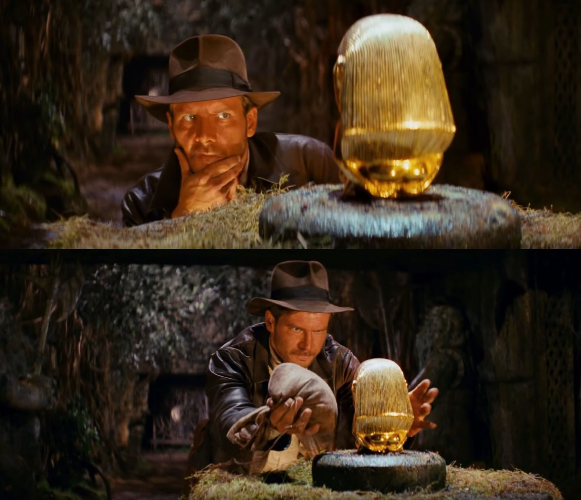
\includegraphics[width=0.5\textwidth]{images/compare-swap.png}
\end{center}

Test-and-Set does not work for the general, counting semaphore.

Alternative: \alert{compare-and-swap} (or compare-and-exchange).

\end{frame}

\begin{frame}[fragile]
\frametitle{Comparing and Swapping}

\begin{lstlisting}[language=C]
int compare_and_swap( int * value, int old_value, int new_value ) {
  if ( *value == old_value ) {
    *value = new_value;
    return old_value;
  }
  return *value;
}
\end{lstlisting}

\end{frame}

\begin{frame}[fragile]
\frametitle{Comparing and Swapping}

And to make use of it in trying to decrement a semaphore:

\begin{lstlisting}[language=C]
int old = 1;
while (true) {
  int actual = compare_and_swap( sem, old, old - 1 );
  if ( actual == old ) {
    old = old - 1;
    break;
  } else {
    old = actual;
  }
}
/* WAIT FOR OUR TURN */
/* critical section */
while (true) {
  int actual = compare_and_swap( sem, old, old + 1 );
  if ( actual == old ) {
    break;
  } else {
    old = actual;
  }
}
\end{lstlisting}

\end{frame}

\begin{frame}
\frametitle{It Took How Many Tries?}

We will eventually succeed, even if it takes an arbitrary amount of time.

 It might be possible for a thread to be so unlucky it never gets a turn, but let's just say that this does not happen.

The initial guess for \texttt{old} can certainly be wrong; the initial attempt to set it will fail and we'll get the correct value.

Need to use CAS for decrementing also!

\end{frame}

\begin{frame}
\frametitle{Wait, Why?}

Alternative: if there is appropriate hardware support, do an atomic increment or atomic decrement.

That prevents a scenario where multiple attempts are necessary to get the value. 

\end{frame}

\begin{frame}
\frametitle{Terms and Conditions Apply}

\begin{center}
	
\includegraphics[width=0.5\textwidth]{images/legaleagle.png}
\end{center}

There is the big ~~\texttt{WAIT FOR OUR TURN} ~~ comment there...

Uh... how \textit{do} we wait for it?

\end{frame}

\begin{frame}
\frametitle{The Future is Now}

Earlier: if we don't get the result we want, the OS blocks the thread.

No details were provided as to how that happens; just hand-waving.

\begin{center}
	
\includegraphics[width=0.5\textwidth]{images/tomorrow.png}
\end{center}

\end{frame}

\begin{frame}
\frametitle{Blocking and Unblocking}

So you want to lock a mutex or wait on a semaphore...

There was a system call; it had a TAS, CAS, or atomic operation.

If this was a trylock call, they don't get blocked; skip this section.

\end{frame}

\begin{frame}
\frametitle{Block On}

Blocking a thread is easy for the operating system.

\begin{center}
	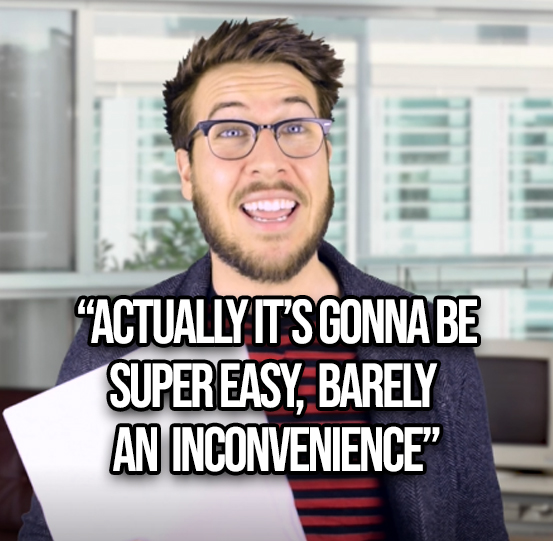
\includegraphics[width=0.4\textwidth]{images/supereasy.jpg}
\end{center}

Change the status to be blocked and choose another thread to run.

\end{frame}

\begin{frame}
\frametitle{Blocked Threads Go Where?}

Marking a thread as blocked or moving it to a ``blocked'' queue is insufficient.

We will need some way of knowing that this thread is blocked on the particular semaphore or mutex it was accessing.

Maybe the mutex/semaphore has its own queue?

\end{frame}

\begin{frame}
\frametitle{Unblocking}

Whichever thread did lock the mutex will want to unlock it or some thread will post on a semaphore.

Counting semaphore: always increase counter, unblock a thread waiting.

Mutex: change the counter only if no thread waiting, otherwise unblock.

\end{frame}

\begin{frame}
\frametitle{Who's Waiting?}

This prompts immediately the question of what thread should be unblocked when an unlock or post event occurs. 

Again, that's a scheduling decision, but you could choose a simple and ``fair'' approach of just taking the first thread in the queue. 

This might not be optimal. Why?

\end{frame}

\begin{frame}
\frametitle{On the Other Hand}

The first-come-first-served approach does prevent the possibility of starvation, as each thread will eventually get a turn.

But just basing it on priority may not be enough?

Could we try to detect deadlock risk?

\end{frame}

\begin{frame}
\frametitle{Get to the Choppa}

The thread that's unblocked is marked as ready to run again.\\
\quad Moved to ready queue?

And at this point it is a scheduling decision: which thread continues execution. 

But we knew that from doing all this from the application developer point of view.

\end{frame}

\begin{frame}
\frametitle{Carry On Then}

When a thread is unblocked it resumes its execution at the return of the system call and will proceed as expected.

That was easier than expected!

\end{frame}

\begin{frame}
\frametitle{RW Locks}

Previously: build up the RW lock using combo of semaphores/mutex.


It's likely more efficient to have a self-contained construct that meets the goal.

A simple counter is probably insufficient. Why?

\end{frame}

\begin{frame}
\frametitle{Counter}

If the counter is currently 1, is that a reader or a writer thread?

So let's have two counters, shall we? One for readers and one for writers.

But things get interesting depending on whether you care about writer priority.

\end{frame}

\begin{frame}
\frametitle{Equality for All}

How should this work if we don't give priority to either side?

\end{frame}

\begin{frame}
\frametitle{Two Counters?}

At first we might consider two counters; one for readers and one for writers. 

If the readers counters is 7, is that seven readers currently in the room or seven readers waiting to enter? 

It's hard to know and we'll need some more accounting.

\end{frame}

\begin{frame}
\frametitle{I have a cunning plan...}

We talked about the light bulb analogy for the way of understanding the reader-writer lock...

\begin{center}
	
\includegraphics[width=0.2\textwidth]{images/idea.png}
\end{center}

\end{frame}

\begin{frame}
\frametitle{Use the Light Bulb}

Idea: a boolean variable that says whether the lights are on. 

Then a counter could be used to keep track of the number of readers currently in the room. 

The reader-writers lock can have associated reader and writer queues. 

\end{frame}

\begin{frame}
\frametitle{Reader Does What?}

Reader: try to set light switch from 0 to 1 with TAS.

If they succeeded, they're the first reader: proceed.

If they failed, why? Readers or writers?

\end{frame}

\begin{frame}
\frametitle{Reader Does What?}

When the reader is done, decrement.

If it falls to zero, unblock a writer if one waiting...\\
\quad Otherwise set light switch to 0.

\end{frame}

\begin{frame}
\frametitle{Writer Does What?}

If a writer wants to enter the room, try to change the light switch from 0 to 1. 

If the writer succeeds, it can proceed. 

If it fails, block the writer. 

\end{frame}

\begin{frame}
\frametitle{Writer Does What?}

When the writer is done, unblock either all waiting readers or a writer. 


Note that it's \textit{all} the readers!

Can we prioritize writers here?

\end{frame}

\begin{frame}
\frametitle{Priority to Writers}

Yes, writers always choose writers at the end.

There is a risk of starvation -- is that okay?

\end{frame}

\begin{frame}
\frametitle{Writer Priority}

That's not quite what we wanted. 

Goal: when a writer is waiting, no new readers are allowed to enter the room. 

How would we go about that? 

\end{frame}

\begin{frame}
\frametitle{Writer Priority}

When a reader wants to enter the room, take a look at the state of the waiting queue for writers. 

If there is one, even if we would normally let the reader proceed, block the reader thread.

\begin{center}
	
\includegraphics[width=0.5\textwidth]{images/sorcery.jpg}
\end{center}

\end{frame}

\begin{frame}
\frametitle{Is This Atomic?}

The logic requires us to try to change the light switch and also to maybe modify the counter and then decide based on that.

That's not atomic!

We may need a mutex internally here.

\end{frame}

\begin{frame}
\frametitle{On the Right Track?}

 We discussed the implementation of a RW spinlock in Linux:

\begin{center}
	\begin{tabular}{l|l|l}
		\textbf{Counter} & \textbf{Flag} & \textbf{Interpretation}                                     \\\hline
		0                & 1             & The spinlock is released and available.                     \\
		0                & 0             & The spinlock has been acquired for writing.                 \\
		$n$ ($n > 0$)    & 0             & The spin lock has been acquired for reading by $n$ threads. \\
		$n$ ($n > 0$)    & 1             & Invalid state.                                              \\
	\end{tabular}
\end{center}

I'd say this validates our idea for how to implement RW Locks...

\end{frame}

\end{document}

